\documentclass[10pt]{beamer}
\usepackage[english]{babel}
\usepackage[utf8]{inputenc}
\usepackage[T1]{fontenc}
\usepackage{helvet}
\usepackage{ragged2e}
%-------------------------------------------------------
% INFORMATION IN THE TITLE PAGE
%-------------------------------------------------------

\newcommand{\cstitle}{\textbf{Bioinformatics}}
\subtitle[]{BLAST}
\newcommand{\cscourseCode}{1005155}
\newcommand{\csauthor}{MSc. Vicente Machaca Arceda}
\institute[UNSA]{Universidad Nacional de San Agustín de Arequipa}
\newcommand{\csemail}{vmachacaa@unsa.edu.pe}
\newcommand{\instituteabr}{UNSA}
\newcommand{\nameUp}{ICC Fase 1}
\date{\today}
\title[\cscourseCode]{\cstitle}
\author{\csauthor}
%%%%%%%%%%%%%%%%%

%-------------------------------------------------------
% CHOOSE THE THEME
%-------------------------------------------------------
\def\mycmd{0} % CS THEME
%\def\mycmd{1} % MYTHEME
%-------------------------------------------------------


\if\mycmd1
\usetheme[]{Feather}
\newcommand{\chref}[2]{	\href{#1}{{\usebeamercolor[bg]{Feather}#2}} }
\else
\usepackage{csformat}
\fi

\newcommand{\1}{
	\setbeamertemplate{background}{
		
\includegraphics[width=\paperwidth,height=\paperheight]{img/1}
		\tikz[overlay] \fill[fill opacity=0.75,fill=white] (0,0) rectangle (-\paperwidth,\paperheight);
	}
}



%-------------------------------------------------------
% THE BODY OF THE PRESENTATION
%-------------------------------------------------------

\begin{document}
	
	
	\AtBeginSubsection[]
	{
		\begin{frame}
			\frametitle{Table of Contents}
			\tableofcontents[currentsubsection]
		\end{frame}
	}
	
	
	%-------------------------------------------------------
	% THE TITLEPAGE
	%-------------------------------------------------------
	
	\if\mycmd1 % MY THEME
	\1{
		\begin{frame}[plain,noframenumbering] 
			\titlepage 
		\end{frame}}
		\else % CS THEME
		\maketitle
		\fi

%-------------------------------------------------------
%-------------------------------------------------------
\begin{frame}{Table of Contents}
\tableofcontents
\end{frame}
%-------------------------------------------------------
%-------------------------------------------------------

%%%%%%%%%%%%%%%%%%%%%%%%%%%%%%%%%%%%%%%%%%%%%%%%%%%%%%%%%%%%%%%%%%%%%%%%%%%%%%%%%%%%%%%%%%%%%%%%%%%%%%%%%%%%%%%%
%%%%%%%%%%%%%%%%%%%%%%%%%%%%%%%%%%%%%%%%%%%%%%%%%%%%%%%%%%%%%%%%%%%%%%%%%%%%%%%%%%%%%%%%%%%%%%%%%%%%%%%%%%%%%%%%
\section{Introduction}
%%%%%%%%%%%%%%%%%%%%%%%%%%%%%%%%%%%%%%%%%%%%%%%%%%%%%%%%%%%%%%%%%%%%%%%%%%%%%%%%%%%%%%%%%%%%%%%%%%%%%%%%%%%%%%%%
%%%%%%%%%%%%%%%%%%%%%%%%%%%%%%%%%%%%%%%%%%%%%%%%%%%%%%%%%%%%%%%%%%%%%%%%%%%%%%%%%%%%%%%%%%%%%%%%%%%%%%%%%%%%%%%%

%%%%%%%%%%%%%%%%%%%%%%%%%%%%%%%%%%%%%%%%%%%%%%%%%%%%%%%%%%%%%%%%%%%%%%%%%%%%%%%%%%%%%%%%%%%%%%%%%%%%%%%%%%%%%%%%
%%%%%%%%%%%%%%%%%%%%%%%%%%%%%%%%%%%%%%%%%%%%%%%%%%%%%%%%%%%%%%%%%%%%%%%%%%%%%%%%%%%%%%%%%%%%%%%%%%%%%%%%%%%%%%%%
\subsection{Objectives}
%%%%%%%%%%%%%%%%%%%%%%%%%%%%%%%%%%%%%%%%%%%%%%%%%%%%%%%%%%%%%%%%%%%%%%%%%%%%%%%%%%%%%%%%%%%%%%%%%%%%%%%%%%%%%%%%
%%%%%%%%%%%%%%%%%%%%%%%%%%%%%%%%%%%%%%%%%%%%%%%%%%%%%%%%%%%%%%%%%%%%%%%%%%%%%%%%%%%%%%%%%%%%%%%%%%%%%%%%%%%%%%%%

%-------------------------------------------------------
%-------------------------------------------------------
\begin{frame}{Introduction}{Objectives}
\begin{itemize}
    \item<1-> Understand the importance of sequence alignment in Bioinformatics. 
    \item<2-> Understand and implement BLAST algorithm.
  \end{itemize}
\end{frame}
%-------------------------------------------------------
%-------------------------------------------------------


%%%%%%%%%%%%%%%%%%%%%%%%%%%%%%%%%%%%%%%%%%%%%%%%%%%%%%%%%%%%%%%%%%%%%%%%%%%%%%%%%%%%%%%%%%%%%%%%%%%%%%%%%%%%%%%%
%%%%%%%%%%%%%%%%%%%%%%%%%%%%%%%%%%%%%%%%%%%%%%%%%%%%%%%%%%%%%%%%%%%%%%%%%%%%%%%%%%%%%%%%%%%%%%%%%%%%%%%%%%%%%%%%
\subsection{Requeriments of database searching}
%%%%%%%%%%%%%%%%%%%%%%%%%%%%%%%%%%%%%%%%%%%%%%%%%%%%%%%%%%%%%%%%%%%%%%%%%%%%%%%%%%%%%%%%%%%%%%%%%%%%%%%%%%%%%%%%
%%%%%%%%%%%%%%%%%%%%%%%%%%%%%%%%%%%%%%%%%%%%%%%%%%%%%%%%%%%%%%%%%%%%%%%%%%%%%%%%%%%%%%%%%%%%%%%%%%%%%%%%%%%%%%%%

%-------------------------------------------------------
%-------------------------------------------------------
\begin{frame}{Requeriments of database searching}
	\begin{block}{}
		\begin{itemize}
			\item \textbf{Sensitivity}.- Ability to find as many correct hits possible (true positives).
			\item \textbf{Selectivity/Specificity}.- Ability to exclude incorrect hits (false positives).
			\item \textbf{Speed}.- Time to take the results.
		\end{itemize}
			
	\end{block}
\end{frame}
%-------------------------------------------------------
%-------------------------------------------------------




%%%%%%%%%%%%%%%%%%%%%%%%%%%%%%%%%%%%%%%%%%%%%%%%%%%%%%%%%%%%%%%%%%%%%%%%%%%%%%%%%%%%%%%%%%%%%%%%%%%%%%%%%%%%%%%%
%%%%%%%%%%%%%%%%%%%%%%%%%%%%%%%%%%%%%%%%%%%%%%%%%%%%%%%%%%%%%%%%%%%%%%%%%%%%%%%%%%%%%%%%%%%%%%%%%%%%%%%%%%%%%%%%
\section{BLAST}
%%%%%%%%%%%%%%%%%%%%%%%%%%%%%%%%%%%%%%%%%%%%%%%%%%%%%%%%%%%%%%%%%%%%%%%%%%%%%%%%%%%%%%%%%%%%%%%%%%%%%%%%%%%%%%%%
%%%%%%%%%%%%%%%%%%%%%%%%%%%%%%%%%%%%%%%%%%%%%%%%%%%%%%%%%%%%%%%%%%%%%%%%%%%%%%%%%%%%%%%%%%%%%%%%%%%%%%%%%%%%%%%%

%%%%%%%%%%%%%%%%%%%%%%%%%%%%%%%%%%%%%%%%%%%%%%%%%%%%%%%%%%%%%%%%%%%%%%%%%%%%%%%%%%%%%%%%%%%%%%%%%%%%%%%%%%%%%%%%
%%%%%%%%%%%%%%%%%%%%%%%%%%%%%%%%%%%%%%%%%%%%%%%%%%%%%%%%%%%%%%%%%%%%%%%%%%%%%%%%%%%%%%%%%%%%%%%%%%%%%%%%%%%%%%%%
\subsection{Problem}
%%%%%%%%%%%%%%%%%%%%%%%%%%%%%%%%%%%%%%%%%%%%%%%%%%%%%%%%%%%%%%%%%%%%%%%%%%%%%%%%%%%%%%%%%%%%%%%%%%%%%%%%%%%%%%%%
%%%%%%%%%%%%%%%%%%%%%%%%%%%%%%%%%%%%%%%%%%%%%%%%%%%%%%%%%%%%%%%%%%%%%%%%%%%%%%%%%%%%%%%%%%%%%%%%%%%%%%%%%%%%%%%%

%-------------------------------------------------------
%-------------------------------------------------------
\begin{frame}{Problem}
	\begin{figure}[]
		\centering
		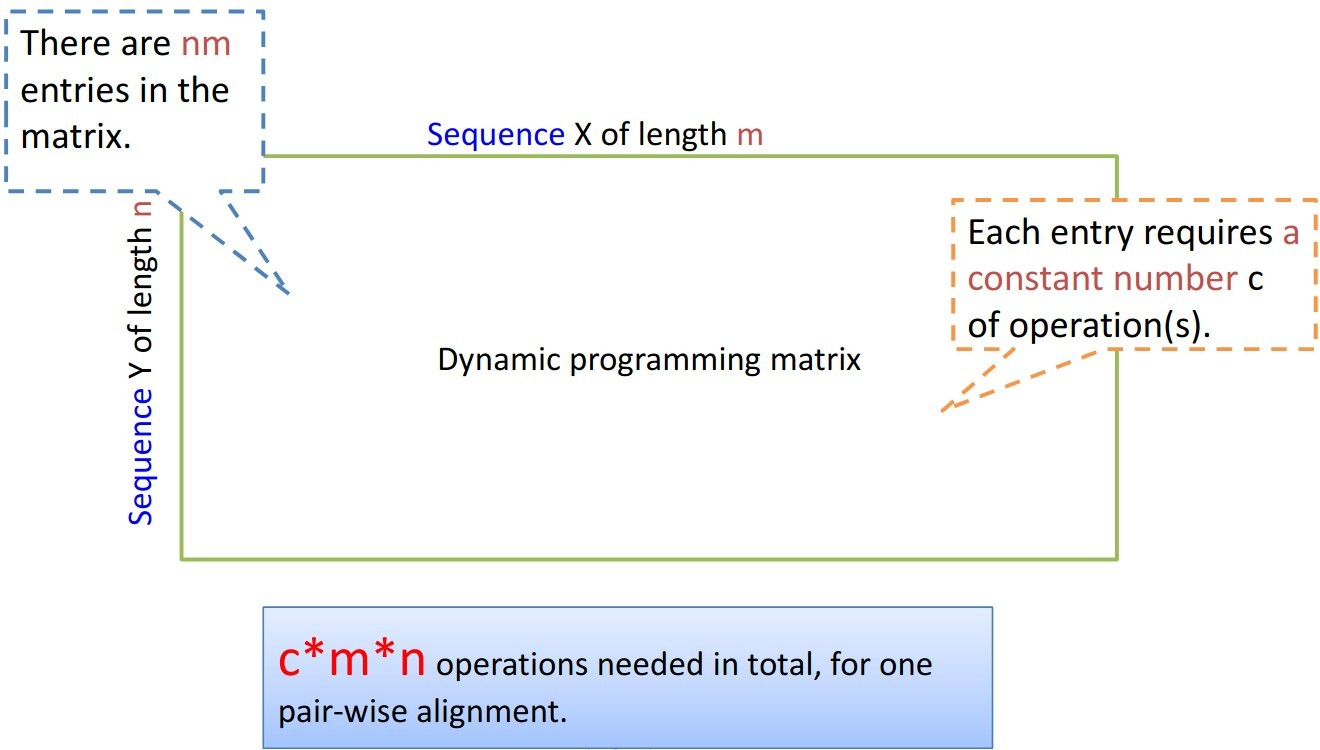
\includegraphics[width=\textwidth,keepaspectratio]{img/alignment/blast1}
		\label{img:uniprot}
		%\caption{Tool for pairwise sequence alignment.}
	\end{figure}
\end{frame}
%-------------------------------------------------------
%-------------------------------------------------------

%%%%%%%%%%%%%%%%%%%%%%%%%%%%%%%%%%%%%%%%%%%%%%%%%%%%%%%%%%%%%%%%%%%%%%%%%%%%%%%%%%%%%%%%%%%%%%%%%%%%%%%%%%%%%%%%
%%%%%%%%%%%%%%%%%%%%%%%%%%%%%%%%%%%%%%%%%%%%%%%%%%%%%%%%%%%%%%%%%%%%%%%%%%%%%%%%%%%%%%%%%%%%%%%%%%%%%%%%%%%%%%%%
\subsection{BLAST algorithm}
%%%%%%%%%%%%%%%%%%%%%%%%%%%%%%%%%%%%%%%%%%%%%%%%%%%%%%%%%%%%%%%%%%%%%%%%%%%%%%%%%%%%%%%%%%%%%%%%%%%%%%%%%%%%%%%%
%%%%%%%%%%%%%%%%%%%%%%%%%%%%%%%%%%%%%%%%%%%%%%%%%%%%%%%%%%%%%%%%%%%%%%%%%%%%%%%%%%%%%%%%%%%%%%%%%%%%%%%%%%%%%%%%

%-------------------------------------------------------
%-------------------------------------------------------
\begin{frame}{BLAST}{Definition}
	\begin{block}{Basic Local alignment Search Tool}
		Proposed by Altschul in 1990 \cite{altschul1990basic}, it use heuristics to reduce time processing in dynamic programming.
	\end{block}
\end{frame}
%-------------------------------------------------------
%-------------------------------------------------------

%-------------------------------------------------------
%-------------------------------------------------------
\begin{frame}{BLAST}{Algorithm}
	\begin{block}{}
		\begin{itemize}
			\item Given query sequence Q, compile the list of possible words.
			\item For each word, compute a list of neighbors based on a similarity matrix.
			\item Scan database for exact matching (hits) with the list of neighbors. 
			\item Extending hits. 
			\item Evaluating significance of extended hits.
		\end{itemize}
		
		
	\end{block}
\end{frame}
%-------------------------------------------------------
%-------------------------------------------------------

%-------------------------------------------------------
%-------------------------------------------------------
\begin{frame}{BLAST}{Seeding}
	For a given word length \textit{w} (usually 3 for proteins and 11 for nucleotides), slicing the query sequence into multiple continuous \textbf{seed words}.
	
		\begin{figure}[]
		\centering
		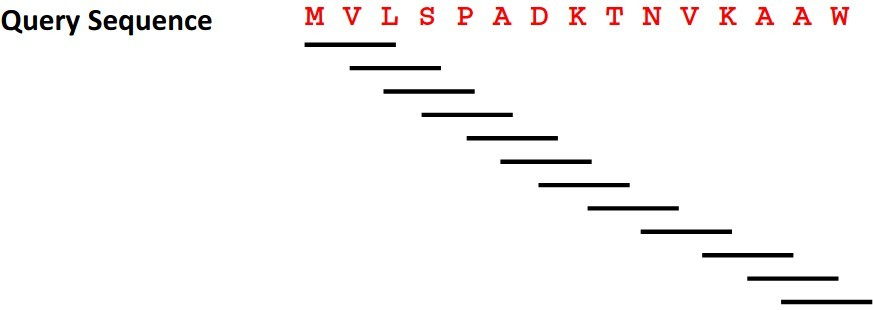
\includegraphics[width=0.8\textwidth,keepaspectratio]{img/alignment/blast2}
		%\label{img:mot2}
		%\caption{Image example in 2 gray levels.}
	\end{figure}
\end{frame}
%-------------------------------------------------------
%-------------------------------------------------------

%-------------------------------------------------------
%-------------------------------------------------------
\begin{frame}{BLAST}{Seeding}
	Examples of words:
	\begin{figure}[]
		\centering
		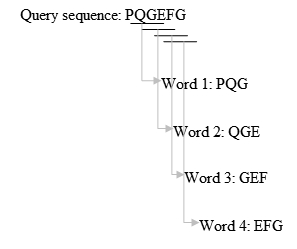
\includegraphics[width=0.6\textwidth,keepaspectratio]{img/alignment/blast3}
		%\label{img:mot2}
		%\caption{Image example in 2 gray levels.}
	\end{figure}
\end{frame}
%-------------------------------------------------------
%-------------------------------------------------------

%-------------------------------------------------------
%-------------------------------------------------------
\begin{frame}{BLAST}{Seeding}
	For each word, compute neighbors ($20^3$ possibilities). Then score the neighbors (BLOSUM62) and choose the ones that its scores are bigger than $T$ ($T = 13$).
	\begin{figure}[]
		\centering
		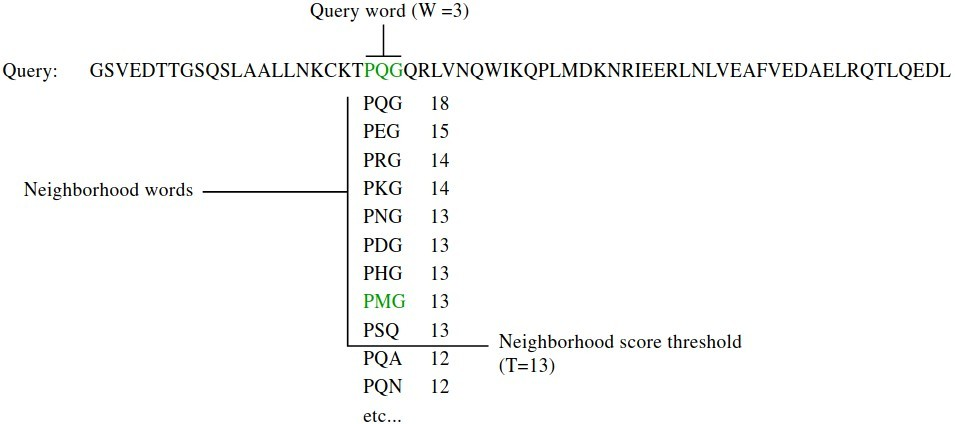
\includegraphics[width=\textwidth,keepaspectratio]{img/alignment/blast6}
		%\label{img:mot2}
		%\caption{Image example in 2 gray levels.}
	\end{figure}
\end{frame}
%-------------------------------------------------------
%-------------------------------------------------------

%-------------------------------------------------------
%-------------------------------------------------------
\begin{frame}{BLAST}{Search a sequence database}
	In sequences database, locate the neighbors. This matches are named: hits.
	\begin{itemize}
		\item HashTable: direct addressing method.
		\item Deterministic finite automaton/finite state machine: much faster.
	\end{itemize}

	\begin{figure}[]
		\centering
		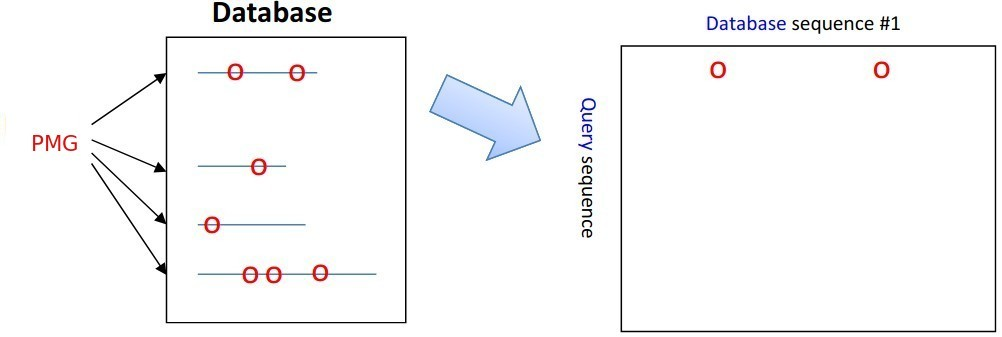
\includegraphics[width=0.8\textwidth,keepaspectratio]{img/alignment/blast4}
		%\label{img:mot2}
		%\caption{Image example in 2 gray levels.}
	\end{figure}
\end{frame}
%-------------------------------------------------------
%-------------------------------------------------------

%-------------------------------------------------------
%-------------------------------------------------------
\begin{frame}{BLAST}{Extending}
	Extend the hit until the score of the alignment drops
	below a threshold (22 for proteins and 20 for DNA). The resulting alignment is called high-scoring segment pair (HSP)
	\begin{figure}[]
		\centering
		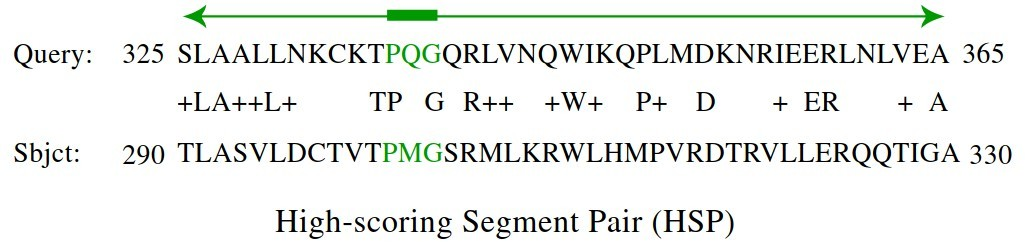
\includegraphics[width=0.8\textwidth,keepaspectratio]{img/alignment/blast10}
		%\label{img:mot2}
		%\caption{Image example in 2 gray levels.}
	\end{figure}
\end{frame}
%-------------------------------------------------------
%-------------------------------------------------------


%-------------------------------------------------------
%-------------------------------------------------------
\begin{frame}{BLAST}{Extending}
	Another example of Extending.
	\begin{figure}[]
		\centering
		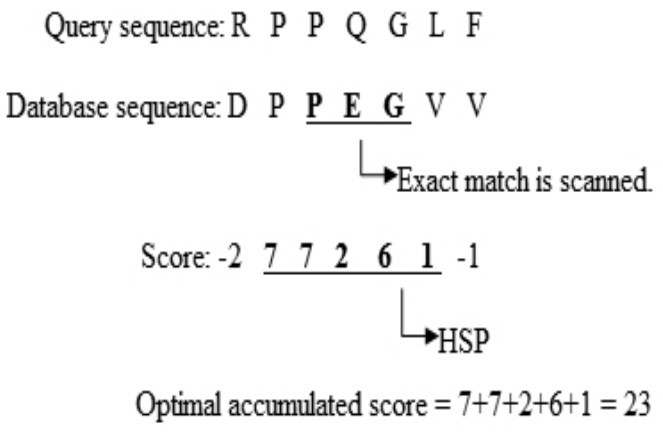
\includegraphics[width=0.8\textwidth,keepaspectratio]{img/alignment/blast7}
		%\label{img:mot2}
		%\caption{Image example in 2 gray levels.}
	\end{figure}
\end{frame}
%-------------------------------------------------------
%-------------------------------------------------------

%-------------------------------------------------------
%-------------------------------------------------------
\begin{frame}{BLAST}{Algorithm}
	
	\begin{figure}[]
		\centering
		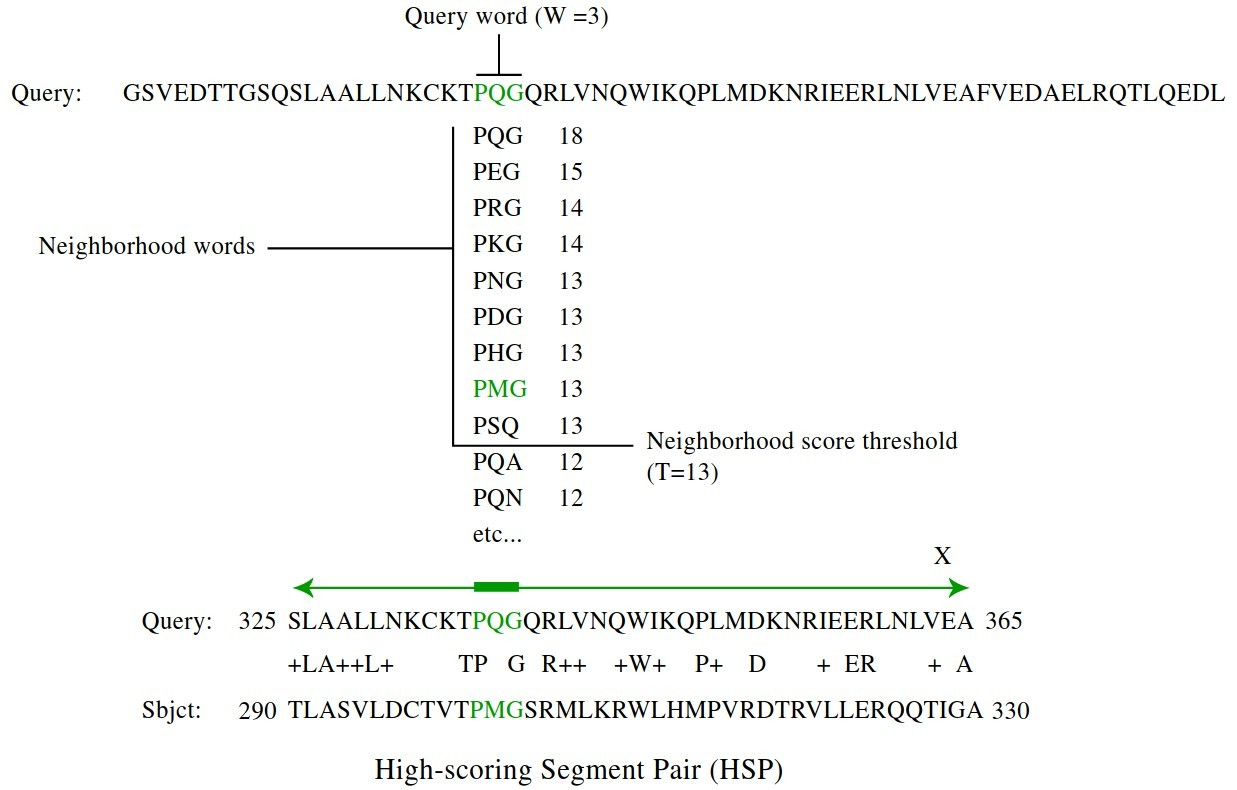
\includegraphics[width=\textwidth,keepaspectratio]{img/alignment/blast9}
		%\label{img:mot2}
		%\caption{Image example in 2 gray levels.}
	\end{figure}
\end{frame}
%-------------------------------------------------------
%-------------------------------------------------------

%-------------------------------------------------------
%-------------------------------------------------------
\begin{frame}{BLAST}{Algorithm}

	\begin{figure}[]
		\centering
		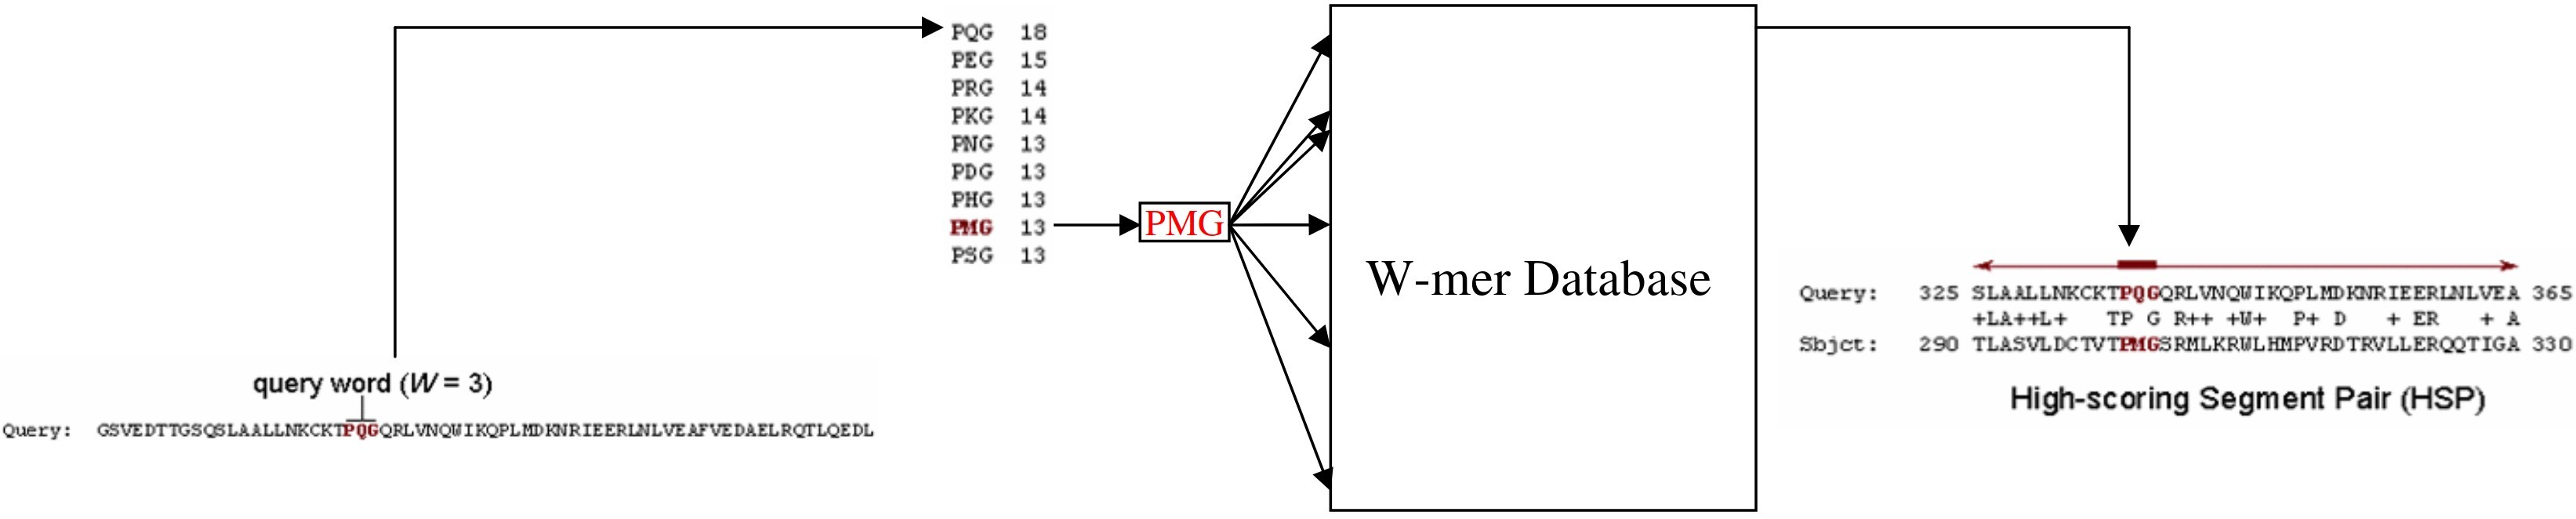
\includegraphics[width=\textwidth,keepaspectratio]{img/alignment/blast8}
		%\label{img:mot2}
		%\caption{Image example in 2 gray levels.}
	\end{figure}
\end{frame}
%-------------------------------------------------------
%-------------------------------------------------------

%-------------------------------------------------------
%-------------------------------------------------------
\begin{frame}{BLAST}{E-value: Significance evaluation}
The \textbf{E-value} provides information about the likelihood that a given sequence match
is purely by chance.
\begin{block}{}
	\[
	E = m*n*p
	\]
\end{block}
where:
\begin{itemize}
	\item $m$: Is the total number of residues in a database.
	\item $n$: Is the number of residues in the query sequence.
	\item $p$: Is the probability that an HSP alignment is a result of
	random chance.

\end{itemize}


\end{frame}
%-------------------------------------------------------
%-------------------------------------------------------



%-------------------------------------------------------
%-------------------------------------------------------
\begin{frame}{BLAST}{E-value: Significance evaluation}
	
	\begin{table}[]
		\begin{tabular}{|l|p{6cm}|}
			\hline
			\textbf{E} & \textbf{Description} \\ \hline
			
			$10 < E  $          & The sequences under consideration  are either unrelated or related by extremely distant relationships.         \\ \hline
			$0.01 < E < 10$          & The match is considered not significant, but
			may hint at a tentative remote homology relationship.          \\ \hline
			$1x10^{-50} < E < 0.01$          & The match can be considered a result		of homology.      \\  \hline  
			$E < 1x10^{-50}$          & There should be an extremely high confidence that the database match is a result of homologous 	relationships. \\  \hline
		\end{tabular}
	\end{table}
		
\end{frame}
%-------------------------------------------------------
%-------------------------------------------------------



%-------------------------------------------------------
%-------------------------------------------------------
\begin{frame}{BLAST}{Bit score: Significance evaluation}
	The \textbf{bit score (S')} measures sequence similarity independent of
	query sequence length and database size and is normalized based on the raw pairwise
	alignment score.
	\begin{block}{}
		\[
		S' = ( \lambda * S - lnK ) / ln2
		\]
	\end{block}
	where:
	\begin{itemize}
		\item $\lambda$: Gumble distribution constant.
		\item $S$: The raw alignment score.
		\item $K$: Constant associated with the scoring matrix used.
		
	\end{itemize}
	
	The higher the bit score, the more	highly significant the match is.
\end{frame}
%-------------------------------------------------------
%-------------------------------------------------------



%-------------------------------------------------------
%-------------------------------------------------------
\if\mycmd1 % MY THEME
\1{
	{\1
		\begin{frame}[plain,noframenumbering]
			%\finalpage{Thank you}
			\begin{figure}[]
				\centering
				
\includegraphics[width=\textwidth,height=0.7\textheight,keepaspectratio]{img/question.png}
				%\label{img:mot2}
				%\caption{Image example in 2 gray levels.}
			\end{figure}
	\end{frame}}
	\else % CS THEME
	\begin{frame}{Questions?}
		\begin{figure}[]
			\centering
			
\includegraphics[width=\textwidth,height=0.7\textheight,keepaspectratio]{img/question.png}
			%\label{img:mot2}
			%\caption{Image example in 2 gray levels.}
		\end{figure}
		
	\end{frame}
	\fi
	%-------------------------------------------------------
	%-------------------------------------------------------

%-------------------------------------------------------
%-------------------------------------------------------
\begin{frame}[allowframebreaks]
	\frametitle{References}
	%\bibliographystyle{amsalpha}
	\bibliographystyle{IEEEtran}
	\bibliography{bibliography.bib}
\end{frame}
%-------------------------------------------------------
%-------------------------------------------------------

\end{document}